\chapter{Java I/O}

 
 \begin{summary}
File handling is a fundamental aspect of programming, allowing developers to read from, write to, and manipulate files.  Java provides two primary APIs for file handling—the traditional java.io package and the more recent java.nio package. Understanding these APIs enables Java developers to efficiently manage data stored in files. 
 \end{summary}
 
 \section{Basics of File Handling}
 
A file system manages access to both the content of files and the metadata about those files.  Files are stored in directories.  The files and directories are accessed by specifying paths.  Paths are either absolute or relative:

\begin{itemize}
\item An absolute path is a path relative to the file system’s root directory. It’s expressed as the root directory symbol followed by a delimited hierarchy of directory names that ends in the target directory or file name.
\item A relative path is a path relative to some other directory. It’s expressed similarly to an absolute path but without the initial root directory symbol. In contrast, it’s often prefixed with one or more delimited “..” character sequences, where each sequence refers to a parent directory.
\end{itemize}

\begin{thm}[java.io.File]
        \url{https://docs.oracle.com/en/java/javase/21/docs/api/java.base/java/io/File.html}
    \end{thm}



\begin{lstlisting}
package be.pxl.ja;

public class Demo01 {

	public static final String SEPARATOR = System.getProperty("file.separator");

	public static void main(String[] args) {
		System.out.println("Current operating system: " + System.getProperty("os.name"));
		System.out.println("File separator: " + SEPARATOR);
		System.out.println("User's home directory: " + System.getProperty("user.home"));
		System.out.println("Current working directory: " + System.getProperty("user.dir"));
	}
}
\end{lstlisting}


On some systems,  Java can compensate for differences such as the direction of the file separator slashes in a pathname. For example,  in the current implementation on Windows platforms,  Java accepts paths with either forward slashes or backslashes.
Thus, using forward slashes will make your application system independent.

\begin{lstlisting}
File file = new File("baeldung/tutorial.txt");
\end{lstlisting}


\begin{lstlisting}
import java.io.File;

public class PartitionSpace
{
   public static void main(String[] args)
   {
      File[] roots = File.listRoots();
      for (File root: roots)
      {
         System.out.println("Partition: " + root);
         System.out.println("Free space on this partition = " +
                            root.getFreeSpace());
         System.out.println("Usable space on this partition = " +
                            root.getUsableSpace());
         System.out.println("Total space on this partition = " +
                            root.getTotalSpace());
         System.out.println("***");
      }
   }
}
\end{lstlisting}


Like the legacy File class, Path also creates an object that may be used to locate a file in a file system.


\begin{thm}[java.nio.file.Path]
        \url{https://docs.oracle.com/en/java/javase/21/docs/api/java.base/java/nio/file/Path.html}
    \end{thm}
    





\begin{lstlisting}
// java.io API
boolean fileExists = file.exists();
boolean fileIsFile = file.isFile();
boolean fileIsDir = file.isDirectory();
boolean fileReadable = file.canRead();
boolean fileWritable = file.canWrite();
boolean fileExecutable = file.canExecute();
boolean fileHidden = file.isHidden();

// java.nio API
boolean pathExists = Files.exists(path);
boolean pathIsFile = Files.isRegularFile(path);
boolean pathIsDir = Files.isDirectory(path);
boolean pathReadable = Files.isReadable(path);
boolean pathWritable = Files.isWritable(path);
boolean pathExecutable = Files.isExecutable(path);
boolean pathHidden = Files.isHidden(path);
\end{lstlisting}



TODO 1.  traverse directory
2. Filenamefilter
3. chat between 2 programs?

1. Basics of File Handling
Introduction to File Class: Understanding the java.io.File class for file and directory pathnames.
2. Reading and Writing Files
Streams: Introduce InputStream and OutputStream for reading from and writing to byte streams (e.g., FileInputStream, FileOutputStream).
Readers and Writers: Discuss Reader and Writer for character stream operations (e.g., FileReader, FileWriter).
Buffering: Explain the use of BufferedReader and BufferedWriter for efficient reading and writing.
3. Working with Directories
Directory Operations: Methods for listing files in a directory, creating directories, etc.
4. Advanced File Operations
Random Access File: Usage of RandomAccessFile class for reading and writing to any location in a file.
5. Java NIO Package
Path and Paths: Introduce Path class as an upgrade to java.io.File.
Files Class: Utilizing Files class for file operations like checking, deleting, copying, moving files, reading, and writing.
File Channels: Discuss FileChannel for reading, writing, mapping, and manipulating a file.
Buffers and ByteBuffers: Understanding how data is buffered in NIO.
Asynchronous File I/O: Introduce AsynchronousFileChannel for asynchronous file operations.
6. Exception Handling in File I/O
Try-with-resources: Best practices for handling exceptions and ensuring that files are properly closed using the try-with-resources statement.
Handling IOExceptions: Strategies for handling IOException.
7. Serialization and Deserialization
Object Streams: Using ObjectInputStream and ObjectOutputStream for object serialization.
8. Practical Exercises and Examples
File Copy: Implement a program to copy a file.
File Browser: Create a simple console-based or GUI file browser.
Text File Processing: Read a text file, process its content, and write the output to another file.
9. Best Practices
File Handling Best Practices: Discuss best practices in file handling such as closing resources, handling exceptions, and ensuring efficient data processing.


 
 \section{Toegang tot bestanden en directories}
 
Een bestandsysteem bevat een verzameling van directories of mappen. Iedere directory bevat vervolgens subdirectories en eventueel bestanden.

Het pad naar een bestand, vanaf de root bekeken, is afhankelijk van het besturingssysteem.

\begin{table}[h!]
\centering
\begin{tabularx}{\textwidth}{| l | X |}
 \hline
 Besturingssysteem & Absoluut pad\\ 
 \hline
 Mac OS X & /Users/mark/courses/JavaAdvanced/Car.java \\
 Windows & C:\textbackslash public\textbackslash html\textbackslash javafaq\textbackslash index.html\\
 Unix & /home/mark/courses/slides.pdf \\
 \hline
 \end{tabularx}
 \end{table}
 
Java is platformonafhankelijk. De code om een bestand te lezen op Mac OS X zal dus identiek zijn als op Windows of Unix. Je maakt als ontwikkelaar gebruik van platformonafhankelijke interfaces. De achterliggende implementatie is afgeschermd voor de ontwikkelaar.
 
Laat ons eerst eens kijken naar het scheidingsteken dat we gebruiken om het pad op te bouwen.
Dit scheidingsteken kunnen we opvragen door systeemeigenschappen te gebruiken.  Naast de systeemeigenschap (system property) ``file.separator'' zijn er nog enkele handige waarden die je in je programma kan gebruiken.



Wanneer je dit programma uitvoert op Mac OS X krijg je bijvoorbeeld de volgende output:
\begin{verbatim}
Current operating system: Mac OS X
File separator: /
User's home directory: /Users/mark
Current working directory: /Users/mark/PXL/JavaAdv/JavaIO
\end{verbatim}

En op het Windows besturingssysteem:
\begin{verbatim}
Current operating system: Windows 10
File separator: \
User's home directory: C:\Users\20003575
Current working directory: C:\Users\20003575\Documents\PXL\JavaAdv\JavaIO
\end{verbatim}

Maar nu terug naar onze initi\"ele vraag: Hoe kunnen we het pad naar een directory of bestand samenstellen?

Absolute paden zijn afhankelijk van het besturingssysteem en kunnen dus bugs en problemen veroorzaken. Je moet dus hardgecodeerde, absolute paden vermijden in je programma's. Best stel je paden at runtime samen door gebruik te maken van systeemeigenschappen en input van de gebruiker.

We bestuderen in dit hoofdstuk interfaces en klassen uit \textit{java.io} en \textit{java.nio}. 
We gaan klassen uit de originele \textit{java.io} library gebruiken om bestanden te lezen en te schrijven. De nieuwere library \textit{java.nio} biedt ons een aantal klassen die het werken met bestanden eenvoudiger maken. \textit{nio} staat voor non-blocking IO. Deze non-blocking manier om bestanden te lezen en te schrijven valt buiten de scope van deze cursus.

Starten doen we met een aantal klassen uit het package \textit{java.nio.file}.

\begin{itemize}
\item De klasse \textbf{FileSystem}: stelt het onderliggend bestandssysteem voor en zorgt ervoor dat er Path-objecten gemaakt kunnen worden.
\item De interface \textbf{Path}: wordt gebruikt om een bestand of directory in een bestandssysteem te localiseren.
\item De klasse \textbf{Files}: deze klasse voorziet static methoden om bewerkingen met bestanden en directories uit te voeren.
\end{itemize}

\subsection{De klasse FileSystem en de interface Path}

Een Path-object cre\"eer je door de static methode \textit{of} van de interface Path aan te roepen. 

\begin{figure}[H]
  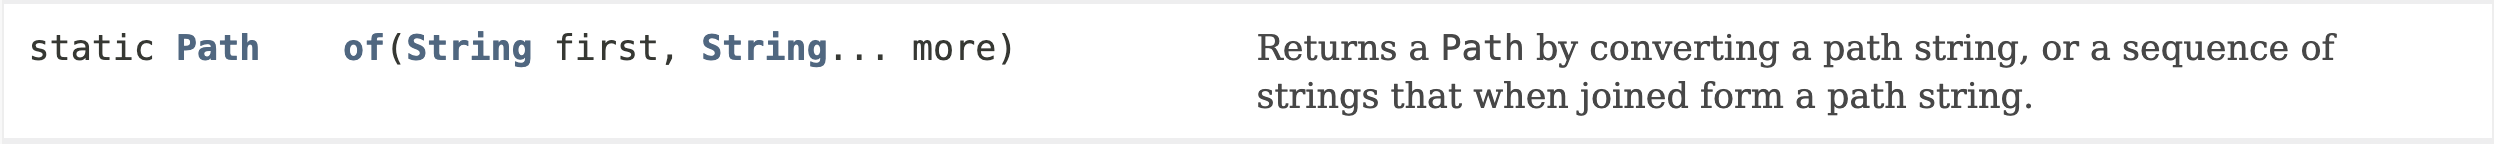
\includegraphics[width=\linewidth]{images/h8/path_of.png}
  \caption{Static methode of in de interface Path}
  \label{fig:paths}
\end{figure}

Achterliggend zal een object van de klasse FileSystem gebruikt worden om Path-objecten te cre\"eeren. FileSystem is wat we noemen een ``factory'' voor Path-objecten. De concrete klasse van een aangemaakt Path-object is afhankelijk van het besturingssysteem.

\begin{lstlisting}
import java.nio.file.FileSystem;
import java.nio.file.FileSystems;
import java.nio.file.Files;
import java.nio.file.Path;

public class Demo02 {

	public static void main(String[] args) {
		FileSystem defaultFileSystem = FileSystems.getDefault();
		System.out.println(defaultFileSystem.getClass());
		for (Path rootDirs: defaultFileSystem.getRootDirectories()) {
			System.out.println(rootDirs);
		}
		Path srcDir = Path.of(System.getProperty("user.dir"), "src");
		System.out.println(srcDir.toAbsolutePath());
		System.out.println(srcDir.getClass().getName());
		System.out.println(Files.isDirectory(srcDir));
	}

}
\end{lstlisting}

Bovenstaand programma geeft volgende uitvoer op een Mac OS X besturingssysteem.

\begin{verbatim}
class sun.nio.fs.MacOSXFileSystem
/
/Users/mark/PXL/JavaAdv/JavaIO/src
sun.nio.fs.UnixPath
true
\end{verbatim}

Volgende uitvoer zal er verschijnen als je het programma uitvoert op een Windows besturingssysteem.

\begin{verbatim}
class sun.nio.fs.WindowsFileSystem
C:\
D:\
C:\Users\20003575\Documents\PXL\JavaAdv\JavaIO\src
sun.nio.fs.WindowsPath
true
\end{verbatim}


\begin{oefening}
Maak via Windows verkenner (of Finder op Mac OS X) de volgende bestandsstructuur aan in directory waarnaar verwezen wordt door de systeemeigenschap \textit{user.home}.

\begin{figure}[H]
  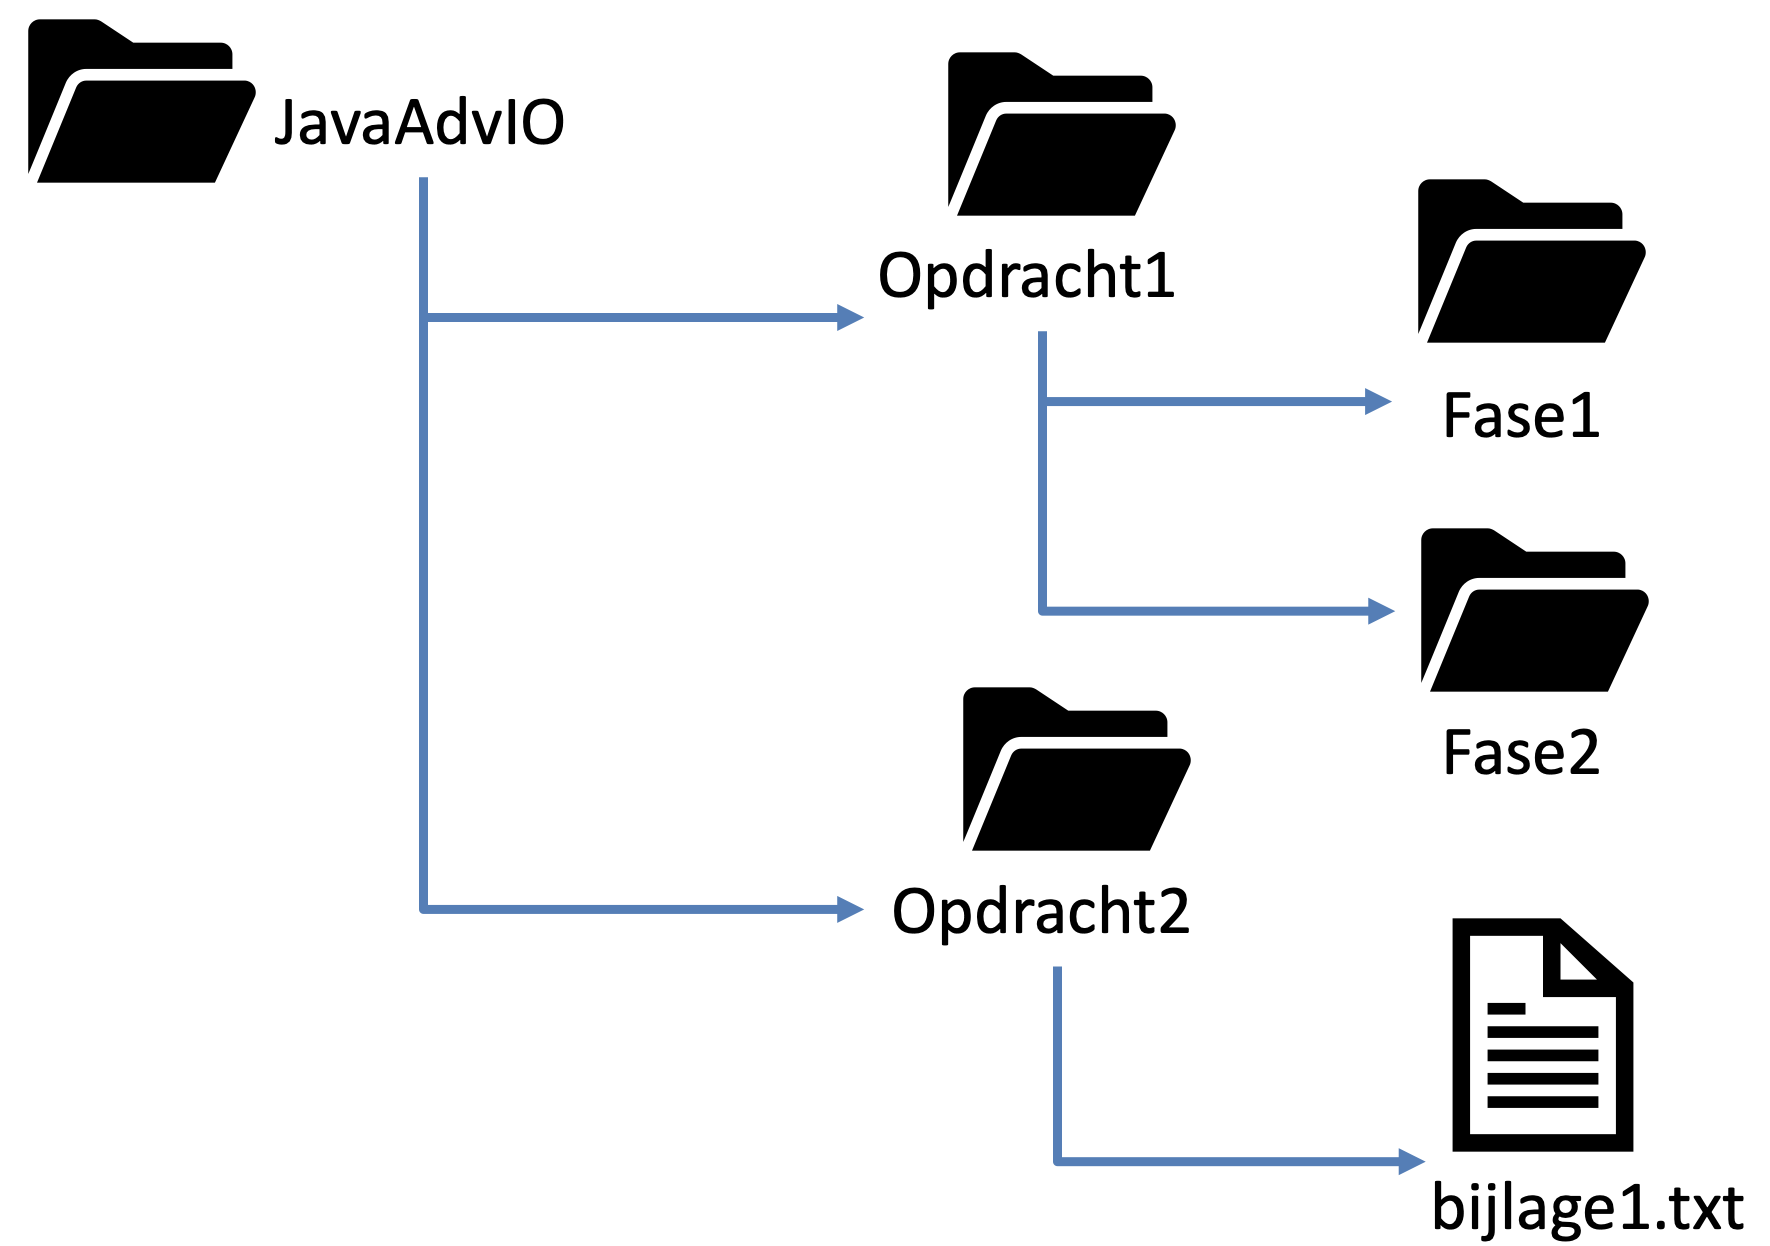
\includegraphics[width=\linewidth]{images/h8/opgave1.png}
  \caption{Bestandsstructuur}
  \label{fig:paths}
\end{figure}

\begin{itemize}
\item Vorm de systeemeigenschap user.home om tot een Path-object.
\item Welke concrete klasse heeft dit Path object?
\item Gebruik de methode resolve() van het Path object, om vanuit de directory user.home het path ``JavaAdvIO/Opdracht1/Fase2'' te volgen.
\item Wat is het resultaat wanneer je volgende methoden uitvoert op het laatst geconstrueerde Path?
\subitem toString()
\subitem getFileName()
\subitem getName(0)
\subitem getNameCount()
\subitem subpath(0,2)
\subitem getParent()
\subitem getRoot()
\end{itemize}
\end{oefening}




\subsection{De utility klasse Files}

De utility klasse \textit{java.nio.files.Files} bezit een groot aantal static methoden om bewerkingen met directories en bestanden uit te voeren.

\begin{oefening}
Zoek de documentatie van de klasse java.nio.files.Files op.
\end{oefening}

\subsubsection{Directories en bestanden aanmaken}

De static methode \textit{createDirectory} kan je gebruiken om een nieuwe directory aan te maken. 


\begin{lstlisting}
import java.io.IOException;
import java.nio.file.Files;
import java.nio.file.Path;

public class Demo03CreatingDirectoriesAndFiles {

	public static void main(String[] args) {
		Path path = Path.of(System.getProperty("user.home"), "JavaAdvIO", "Opdracht3", "bijlage.txt");
		if (Files.notExists(path.getParent())) {
			try {
				Files.createDirectory(path.getParent());
			} catch (IOException e) {
				System.out.println("An error occured while creating directory " + path.getParent());
			}
		}
		if (Files.notExists(path)) {
			try {
				Files.createFile(path);
			} catch (IOException e) {
				System.out.println("An error occured while creating file " + path);
			}
		}
	}

}
\end{lstlisting}

\begin{oefening}
Neem de documentatie er eens bij. Welke exceptions kunnen zich voordoen? Welke van deze exceptions zijn checked? Welke unchecked?
\end{oefening}


\subsubsection{Bestanden lezen (kleine bestanden)}

Als je tekstbestanden met een beperkt aantal regels wil lezen kan je de static methode readAllLines gebruiken.

\begin{lstlisting}
import java.nio.file.Path;
import java.nio.file.Paths;
import java.util.List;
import java.util.Random;

public class Demo04ReadingFiles {
	private static final Random RANDOM = new Random();

	public static void main(String[] args) {
		Path path = Paths.get("resources/small_file_with_text.txt");

		try {
			List<String> text = Files.readAllLines(path);
			System.out.println(text.get(RANDOM.nextInt(text.size())));
		} catch (IOException e) {
			e.printStackTrace();
		}
	}
}
\end{lstlisting}

\subsubsection{Bestanden kopi\"eren}

Je kan eenvoudig bestanden kopi\"eren door gebruik te maken van de static methode copy.

\begin{lstlisting}
import java.io.IOException;
import java.nio.file.Files;
import java.nio.file.Path;
import java.nio.file.Paths;

public class Demo05CopyFiles {

	public static void main(String[] args) {
		Path original = Paths.get("resources/small_file_with_text.txt");
		Path copy = Paths.get("resources", "copy_" + System.currentTimeMillis() + ".txt");
		System.out.println(Files.exists(copy));
		try {
			Files.copy(original, copy);
			System.out.println(Files.exists(copy));
		} catch (IOException e) {
			e.printStackTrace();
		}
	}
}
\end{lstlisting}

\section{Tekstbestanden}


A stream is an ordered sequence of bytes of an arbitrary length. Bytes flow over an output stream from an application to a destination and flow over an input stream from a source to an application.
The java.io package provides several output stream and input stream classes that are descendants of its abstract \textit{OutputStream} and \textit{InputStream} classes.



\begin{oefening}
Exercise: Image Processing in Java - Converting to Grayscale
Objective: Implement a Java program that simulates the process of receiving an image over a network, converting it to grayscale, and then preparing it for transmission. This exercise will help you understand how to manipulate images in memory using ByteArrayInputStream and ByteArrayOutputStream, along with the BufferedImage class for image processing tasks.

Background: In many applications, images need to be processed before they are stored or transmitted. Converting an image to grayscale is a common preprocessing step. In Java, this can be efficiently done using ByteArrayInputStream and ByteArrayOutputStream for in-memory data manipulation, along with BufferedImage for accessing and modifying image pixels.

Requirements:

Read an Image: Simulate receiving an image by loading it from the disk into a byte array. This step mimics downloading an image from the internet.
Convert to Grayscale: Use ByteArrayInputStream to read the byte array into a BufferedImage. Then, convert the image to grayscale by averaging the RGB values of each pixel.
Write the Processed Image: Use ByteArrayOutputStream to write the processed grayscale image to a byte array. This simulates preparing the image for uploading or further processing.
Instructions:

Setup: Start by reading an image file from disk and converting it to a byte array. This simulates receiving image data.
Processing:
Initialize a ByteArrayInputStream with the image byte array.
Use ImageIO.read to convert the byte stream into a BufferedImage.
Implement a method to convert the BufferedImage to grayscale. Iterate over each pixel, calculate the average of the red, green, and blue components, and set the new color for the pixel.
Output:
Initialize a ByteArrayOutputStream.
Use ImageIO.write to write the grayscale BufferedImage to the ByteArrayOutputStream.
You may convert the output stream back to a byte array if you wish to simulate sending the data over a network.
\end{oefening}



If you need to stream characters, you should take advantage of Java’s writer and reader classes, which were designed to support character I/O (they work with char instead of byte). Furthermore, the writer and reader classes take character encodings into account.



BufferedWriter and BufferedReader

BufferedWriter writes text to a character-output stream (a Writer instance), buffering characters so as to provide for the efficient writing of single characters, arrays, and strings. Invoke either of the following constructors to construct a buffered writer:

BufferedWriter(Writer out)
BufferedWriter(Writer out, int size)
The buffer size may be specified, or the default size (8,192 bytes) may be accepted. The default is large enough for most purposes.

BufferedWriter includes a handy void newLine() method for writing a line-separator string, which effectively terminates the current line.

BufferedReader reads text from a character-input stream (a Reader instance), buffering characters so as to provide for the efficient reading of characters, arrays, and lines. Invoke either of the following constructors to construct a buffered reader:

BufferedReader(Reader in)
BufferedReader(Reader in, int size)
The buffer size may be specified, or the default size (8,192 bytes) may be used. The default is large enough for most purposes.

\begin{oefening}

User Input:
Prompt the user to enter a secret message.
Ask for the number of positions to shift in the Caesar cipher (or any simple substitution cipher you choose to use).
Encoding the Message:
Apply the cipher to the message, shifting each letter by the specified number of positions.
Charset Conversion:
Write the encoded message to a file using a specified source charset.
Read the file and convert the charset to a different one, simulating sending the message through a different system.
Decoding the Message:
After converting it back to the original charset, decode the message by reversing the cipher.
Display:
Show the original, encoded, and decoded messages to the user, highlighting how the message remains confidential and intact through the encoding and charset conversion process.

\end{oefening}

\subsection{I/O Streams}

Een I/O stream is een opeenvolging van bytes (8 bits). Je mag I/O streams zeker niet verwarren met de Stream API die we in het vorige hoofdstuk hebben besproken. InputStreams worden gebruikt om gegevens byte per byte aan te bieden aan een Java programma. OutputStreams worden gebruikt om gegevens vanuit een Java programma byte per byte te versturen naar een externe bron (dit kan een bestand zijn, maar ook een andere computer). 
In dit hoofdstuk zijn het bestanden die we als bron of doel van onze I/O streams gebruiken. Je kan tekstbestanden byte per byte gaan inlezen en wegschrijven, maar dit is niet effici\"ent. Karakters worden meestal voorgesteld door meerdere bytes. 
De karakter encodering bepaalt hoeveel bytes er per karakter gebruikt zullen worden. Bij UTF-8 bijvoorbeeld worden 1 tot 4 bytes gebruikt om de karakters voor te stellen. Een alternatief is dus dat je tekstbestanden karakter per karakter gaat inlezen, maar ook dit is niet altiijd effici\"ent.

\subsection{BufferedReader}

De klasse BufferedReader biedt een eenvoudige en effici\"ente manier om grotere tekstbestanden te lezen. Het groepeert (buffert) karakters uit een bestand zodat je het bestand regel per regel kan inlezen. De methode newBufferedReader uit de klasse Files vereenvoudigt het aanmaken van de BufferedReader voor ons.
Het einde van het tekstbestand is bereikt als readLine() \textit{null} geeft.

\begin{figure}[H]
  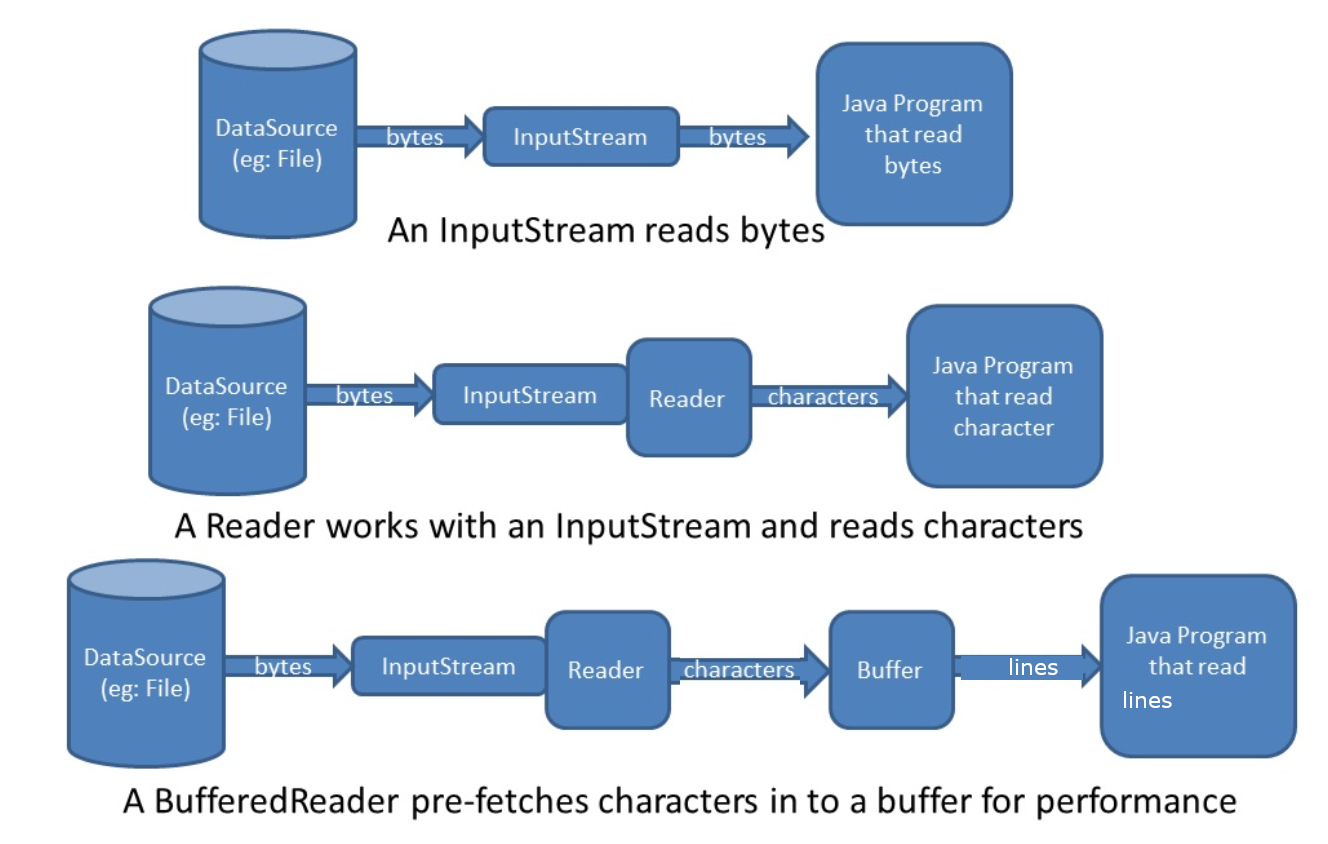
\includegraphics[width=\linewidth]{images/h8/stream_reader.png}
  \caption{InputStream, InputStreamReader en BufferedReader}
  \label{fig:paths}
\end{figure}

\begin{lstlisting}
import java.io.BufferedReader;
import java.io.IOException;
import java.nio.file.Files;
import java.nio.file.Paths;

public class Demo06BufferedReader {

	public static void main(String[] args) {

		try (BufferedReader reader =  Files.newBufferedReader(Paths.get("resources/small_file_with_text.txt"))) {
			String line = null;
			while ((line = reader.readLine()) != null) {
				System.out.println(line);
			}
		} catch (IOException e) {
			e.printStackTrace();
		}
	}
}
\end{lstlisting}

We maken in dit code-voorbeeld gebruik van \textbf{try-with-resources}.
De BufferedReader implementeert namelijk de interface \textit{java.lang.AutoCloseable}. Wanneer je klaar ben met het lezen of schrijven van een bestand, moet je dit namelijk aan het besturingssysteem laten weten. Het besturingssyteem zorgt ervoor dat de toegang tot een bestand goed beheerd wordt zodat er zich geen problemen voordoen wanneer er verschillende programma's gelijktijdig in hetzelfde bestand willen lezen en/of schrijven. Het sluiten van een bestand werd typisch ge\"implementeerd in een \textit{finally-block}. Tegenwoordig zijn veel resources (zoals bestanden) auto-closeable waardoor je deze code niet meer zelf moet schrijven. Door gebruik te maken van try-with-resources wordt het bestand automatisch netjes gesloten zodra het programma klaar is met het lezen of schrijven van het bestand.

\subsection{BufferedWriter}

In plaats van karakter per karakter in een bestand weg te schrijven, gaat BufferedWriter grotere stukken tekst in \'e\'en keer in het bestand wegschrijven. 




\subsection{Character sets}

\begin{lstlisting}
import java.nio.charset.Charset;

public class Demo7DefaultCharset {

	public static void main(String[] args) {

		System.out.println(Charset.defaultCharset().displayName());
	}

}
\end{lstlisting}

Met het bovenstaande programma kan je afdrukken wat de default encoding is die gebruikt wordt om bytes te combineren tot karakters. UTF-8 is de meest gebruikte encoding, maar toch is het een goede gewoonte om de gebruikte karakterset mee te geven als parameter wanneer je een bestand leest of schrijft. Op die manier kan je problemen vermijden.

\begin{lstlisting}
Files.newBufferedWriter(Paths.get("resources/myfile.txt"), Charset.forName("UTF-8"));
\end{lstlisting}


\begin{oefening}
Find out what words are shared by two files, and return the
number of unique words in common. Output the words you find to
a different file.
1 long wordsInCommon ( File file1 , File file2 ) {
2 // TODO implement
3 }

\end{oefening}

\subsection{Het decorator patroon}

De BufferedReader heeft als basis een InputStreamReader waaraan extra functionaliteit wordt toegevoegd, namelijk het bufferen van de karakters. De InputStreamReader vormt op zijn beurt de brug tussen byte streams en character streams. Hij leest bytes en decodeert ze tot karakters door gebruik te maken van een karakterset (Charset).

Wat we bij deze klassen is dat ze ontwikkeld zijn volgens het decorator ontwerppatroon.
In het package \textit{be.pxl.ja.decorator} vind je een eenvoudig voorbeeld van dit ontwerppatroon.

\section{Programma attributen}

Het is een goed idee om Java programma's gemakkelijk configureerbaar te maken. 
Om dit te verwezenlijken zijn parameters bestaande uit een key en een value meestal voldoende. 
In Java gebruik je de klasse \textit{java.util.Properties} om configuratie-bestanden te lezen en weg te schrijven.
Je gebruikt de methode load om een configuratie-bestand in te lezen en store om de eigenschappen weg te schrijven. Met de methode getProperty kan je aan de hand van een key de bijhorende waarde opvragen.

\begin{lstlisting}
import java.io.IOException;
import java.io.InputStream;
import java.io.OutputStream;
import java.nio.file.Files;
import java.nio.file.Path;
import java.util.Properties;
import java.util.Scanner;

public class Demo08ProgramWithProperties {
	private static final String CONFIG_FILE = "resources/config.properties";

	public static void main(String[] args) {
		try(InputStream inputStream = Files.newInputStream(Path.of(CONFIG_FILE))) {
			Properties properties = new Properties();
			properties.load(inputStream);
			System.out.println("Welcome " + properties.getProperty("demo.name") + "!");
			System.out.println("You're mails will be sent to: " + properties.getProperty("demo.email"));
		} catch (IOException e) {
			createProperties();
		}
	}

	private static void createProperties() {
		Scanner scanner = new Scanner(System.in);
		System.out.println("You're using this program for the first time.");
		System.out.println("What's your name:");
		String name = scanner.nextLine();
		System.out.println("What's your company:");
		String company = scanner.nextLine();
		System.out.println("What's your email:");
		String email = scanner.nextLine();
		Properties properties = new Properties();
		properties.setProperty("demo.name", name);
		properties.setProperty("demo.company", company);
		properties.setProperty("demo.email", email);
		try(OutputStream outputStream = Files.newOutputStream(Path.of(CONFIG_FILE))) {
			properties.store(outputStream, "Demo program configuration");
		}
		catch (IOException e) {
			System.out.println("We were not able to save your configuration.");
		}
	}
}
\end{lstlisting}

De eerste keer dat het programma wordt uitgevoerd, is het bestand config.properties bestand nog niet aanwezig is. De gebruiker wordt dan gevraagd om zijn gegevens in te voeren.

\begin{verbatim}
You're using this program for the first time.
What's your name:
Nele
What's your company:
PXL
What's your email:
nele.custers@pxl.be
\end{verbatim}

Je zal zien dat er na het uitvoeren van het programma een bestand \textit{resources/config.properties} is aangemaakt.
Dit bestand bevat de volgende informatie.

\begin{verbatim}
#Demo program configuration
#Tue Nov 17 09:13:51 CET 2020
demo.name=Nele
demo.company=PXL
demo.email=nele.custers@pxl.be
\end{verbatim}
Wanneer je het programma opnieuw opstart, wordt het .properties bestand gelezen en krijg je de volgende output.

\begin{verbatim}
Welcome Nele!
You're mails will be sent to: nele.custers@pxl.be
\end{verbatim}


\section{Byte stream}

Object serialization laat ons toe om de status (de waarden van de eigenschappen) van een object te converteren naar een byte stream. Op die manier kan een object weggeschreven worden in bestand of verstuurd worden over een netwerk.
Deserialization is het omgekeerde proces, waarbij de byte stream terug wordt geconverteerd naar een object.

Enkel objecten van klassen die de interface \textit{Serializable} implementeren kunnen geserialiseerd worden.
Je kan een eigenschap van een klasse \textbf{transient} maken als je de waarde van die eigenschap niet wil serialiseren.

Alle static eigenschappen behoren tot de klasse en niet tot een object, dus de waarden van static field kunnen nooit geserialiseerd worden. 

De klasse ObjectOutputStream die we gebruiken om objecten te schrijven en de klasse ObjectInputStream die we gebruiken om objecten in te lezen, zijn opnieuw implementaties van het decorator patroon. We gaan respectievelijk de klassen FileOutputStream en FileInputStream ``decoreren'' met extra functionaliteit om te werken met volledige objecten in plaats van bytes. 

\subsection{Object serialization}

\begin{lstlisting}
import java.io.FileOutputStream;
import java.io.IOException;
import java.io.ObjectOutputStream;
import java.time.LocalDate;
import java.util.Arrays;
import java.util.List;

public class Demo09Serialization {

	public static void main(String[] args) {
		Student student = new Student("Mare", LocalDate.of(2000, 11, 29));
		student.setGraduationDate(LocalDate.of(2018, 6, 30));
		List<String> animals = Arrays.asList("elephant", "zebra", "donkey");
		try (FileOutputStream file = new FileOutputStream("resources/demo.ser");
		     ObjectOutputStream out = new ObjectOutputStream(file)) {
			out.writeObject(student);
			out.writeObject(animals);
		} catch (IOException ex) {
			System.out.println(ex.getMessage());
		}
	}
}
\end{lstlisting}


\subsection{Object deserialization}

\begin{lstlisting}
import java.io.FileInputStream;
import java.io.IOException;
import java.io.ObjectInputStream;
import java.util.List;

public class Demo09Deserialization {

	public static void main(String[] args) {
		try (FileInputStream file = new FileInputStream("resources/demo.ser");
		     ObjectInputStream in = new ObjectInputStream(file)) {
			Student student = (Student) in.readObject();
			System.out.println(student.getName());
			System.out.println(student.getDateOfBirth());
			List<?> animals = (List<?>) in.readObject();
			//List<String> animals = (List<String>) in.readObject();
			System.out.println(animals.size());
			System.out.println(animals.get(0));
		} catch (IOException ex) {
			System.out.println(ex.getMessage());
		} catch (ClassNotFoundException e) {
			e.printStackTrace();
		}
	}
}
\end{lstlisting}


%\subsection{Audio en afbeeldingen}



\section{Oefeningen}

\begin{oefening}
\textbf{Telefoonboek}\\

Schrijf een programma om telefoonnummers bij te houden.
Wanneer je het programma opstart wordt het bestand phonedirectory.txt ingelezen,
plaats dit dus in een nieuwe folder (bv. resources) in je project. Iedere lijn in het
bestand heeft het volgende formaat: $<naam>;<tel1>;<tel2>;…$
We geven alvast wat startcode voor het printen van het menu.
(PhoneNumbersApp.java)
\begin{itemize}
\item Lees alle lijnen in en steek alle contacten in een Collection, zodat je aan de hand van
een naam de bijhorende telefoonnummers kan zoeken. Let op: er kunnen meerdere
telefoonnummers aan één contact gelinkt worden.
\item Zorg ook voor functionaliteit om telefoongegevens toe te voegen (zie reeds gegeven
code). Als je een telefoonnummer toevoegt dat reeds bestaat voor de gegeven
persoon, gooit het programma een zelfgemaakte exception. (bv.
PhoneDirectoryException). Deze exception moet niet opgevangen worden, dus het
programma mag stoppen met uitvoeren in dit geval.
\item Wanneer je ervoor kiest om het programma af te sluiten, worden alle gegevens eerst
weer weggeschreven in phonedirectory.txt, zodat geen gegevens verloren gaan.
\end{itemize}
\end{oefening}

\begin{oefening}
\textbf{Bank account}\\

Schrijf een applicatie voor het beheren van spaarrekeningen.
Voorzie volgende functionaliteit:
\begin{itemize}
\item Maak een klasse Spaarrekening met de nodige member variabelen (bv. saldo,
naam, nummer, …)
\item Zorg dat instanties van deze klasse als object naar een file geschreven kunnen
worden (Serializable interface)
\item Schrijf in een main methode de code om een volledig Spaarrekening object
naar een file weg te schrijven.
\item Voeg code toe om een spaarrekening object terug uit te lezen uit deze file.
\item Controleer of de member variabelen hun waarde hebben behouden na uitlezen.
\end{itemize}
\end{oefening}


\section{Spring Boot File Handling}





\section{outline}

 Reading and Writing Files
Streams: Introduce InputStream and OutputStream for reading from and writing to byte streams (e.g., FileInputStream, FileOutputStream).
Readers and Writers: Discuss Reader and Writer for character stream operations (e.g., FileReader, FileWriter).
Buffering: Explain the use of BufferedReader and BufferedWriter for efficient reading and writing.
3. Working with Directories
Directory Operations: Methods for listing files in a directory, creating directories, etc.
4. Advanced File Operations
Random Access File: Usage of RandomAccessFile class for reading and writing to any location in a file.
5. Java NIO Package
Path and Paths: Introduce Path class as an upgrade to java.io.File.
Files Class: Utilizing Files class for file operations like checking, deleting, copying, moving files, reading, and writing.
File Channels: Discuss FileChannel for reading, writing, mapping, and manipulating a file.
Buffers and ByteBuffers: Understanding how data is buffered in NIO.
Asynchronous File I/O: Introduce AsynchronousFileChannel for asynchronous file operations.
6. Exception Handling in File I/O
Try-with-resources: Best practices for handling exceptions and ensuring that files are properly closed using the try-with-resources statement.
Handling IOExceptions: Strategies for handling IOException.
7. Serialization and Deserialization
Object Streams: Using ObjectInputStream and ObjectOutputStream for object serialization.
8. Practical Exercises and Examples
File Copy: Implement a program to copy a file.
File Browser: Create a simple console-based or GUI file browser.
Text File Processing: Read a text file, process its content, and write the output to another file.
9. Best Practices
File Handling Best Practices: Discuss best practices in file handling such as closing resources, handling exceptions, and ensuring efficient data processing.


Here are some best practices for reading and writing to files using Java libraries:

Use try-with-resources: When reading or writing to a file, it’s important to properly handle the opening and closing of the file stream. Java 7 introduced the try-with-resources statement which automatically closes the file stream once the code block is executed.
Use buffered streams: Reading or writing large files can be a performance bottleneck. Using buffered streams can help improve performance by reducing the number of I/O operations required.
Handle exceptions: When reading or writing to a file, it’s important to handle any exceptions that may occur. Common exceptions include FileNotFoundException and IOException.
Use appropriate encoding: When reading or writing text files, it’s important to use the appropriate encoding. The default encoding used by Java is usually UTF-8, but this may not be appropriate for all scenarios.
Use relative paths: When working with files, it’s best to use relative paths instead of absolute paths. This makes the code more portable and easier to maintain.
Check for file existence: Before reading or writing to a file, it’s important to check if the file exists. This can be done using the File.exists() method.
Use descriptive file names: When creating new files, it’s important to use descriptive file names that are easy to understand and maintain. This can help prevent naming conflicts and make it easier to find and manage files.
Use constants for file paths: When working with file paths, it’s best to use constants instead of hardcoding the paths in the code. This makes it easier to update file paths in the future.
Close file streams: When finished with a file, it’s important to close the file stream to free up system resources. This can be done using the close() method.
Handle file locking: When working with files, it’s important to handle file locking to prevent multiple processes from accessing the same file at the same time. Java provides a number of methods for handling file locking, including the FileChannel.lock() method.
10. Recent Developments and Additional Resources
Updates in Latest Java Versions: Briefly cover any recent changes or enhancements in file handling in newer Java versions.
External Libraries: Introduction to popular third-party libraries for file handling, if time allows.

